%% body.tex
%% Copyright 2022 skyleaworlder
%
% This work may be distributed and/or modified under the
% conditions of the LaTeX Project Public License, either version 1.3
% of this license or (at your option) any later version.
% The latest version of this license is in
%   http://www.latex-project.org/lppl.txt
% and version 1.3 or later is part of all distributions of LaTeX
% version 2003/12/01 or later.
%
% This work has the LPPL maintenance status "maintained".
%
% This Current Maintainer of this work is skyleaworlder.
%
% This work consists of all the *.tex and *.sty files in
%   https://github.com/TJ-CSCCG/Tongji-Beamer
\section{系统背景}
    % “图片文字并排” 示例
    \begin{frame}{AOSP Frameworks 项目概述}
        \begin{columns}
            \column{.4\textwidth}
            \begin{figure}
                \centering 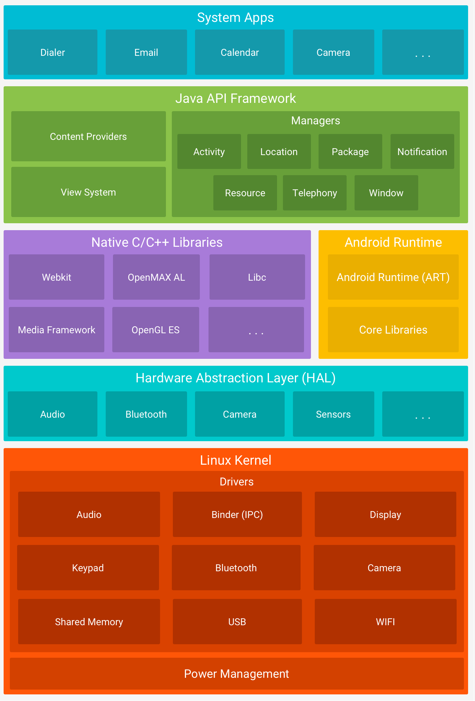
\includegraphics[width=1.45in, height=2in]{contents/figure/AOSP.png}
                \caption{AOSP 项目整体架构}
                \label{fig:aosp}
            \end{figure}

            \column{.65\textwidth}
            \begin{itemize}
                \item Framework 是建立在底层 Android Runtime 和 C/C++ Lib 以及更底层 HAL 之上的,面向应用开发的框架层。 Framework 作为开发者可以直接且完全访问的 Android 系统应用使用的框架 API[1],封装了整个 Android 操作系统的所有功能。
                \item Framework 共由 67 个仓库组成\cite{repo-crawler},主要语言为 Java 以及 C/C++,大版本间有效提交数约为 10 万次,其中 framework/base 是体量最庞大且作用最重要的仓库之一。
            \end{itemize}
        \end{columns}
    \end{frame}

    % “图片文字垂直” 示例
    \begin{frame}{soong 构建系统概述}
        \begin{figure}
            \centering
            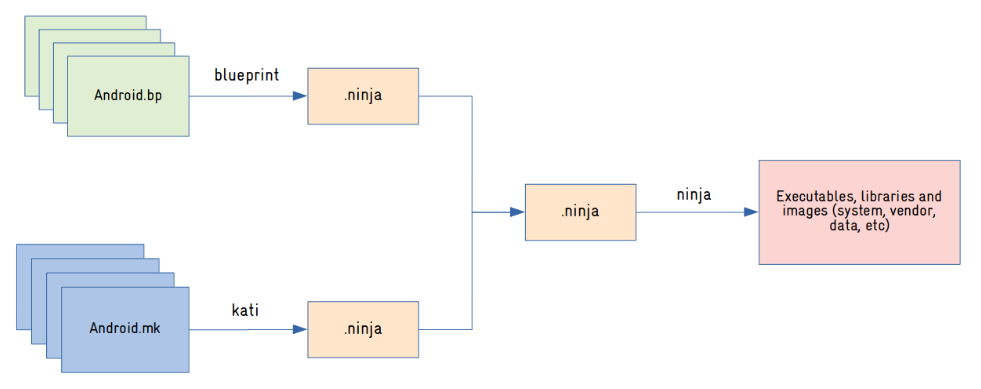
\includegraphics[width=.8\textwidth]{contents/figure/soong.png}
            \label{fig:soong}
        \end{figure}

        \begin{itemize}
            \item \small soong 下生成的完整 Manifest 文件达 2.7 GB,进一步说明 AOSP 体量庞大,难以完全分析。
            \item \small soong 使用底层构建系统 ninja,后者的输入由 soong 生成,具备一定的结构,方便进行基于文本的处理。
        \end{itemize}
    \end{frame}

    % “多图片文字混合” 示例
    \begin{frame}{git 版本控制系统简述}
        \begin{block}{AOSP 下的 git}
            \begin{itemize}
                \item AOSP 中的仓库均使用 git 作为版本控制系统。
                \item git 中存储了每一次提交的代码变更。如:git diff <a-id> <b-id> 可以得到 a 与 b 版本间的文本差异。
                \item 关于变更,git 仅存储了文本 / 二进制差异,并不存在更复杂的、有关源代码的数据结构。
            \end{itemize}
        \end{block}

        \small 对于软件变更分析,通常需要基于给定的两个不同的版本展开分析。对于 git 版本控制系统而言,则是需要给出两个可用于代表提交的 Hash ID。

        \small 通过 git 内部的存储结构,可以获得两版本间涉及变更的文件名以及变更内容。这有助于进一步展开对模块间以及模块内部的依赖分析。
    \end{frame}

\section{解决方法与过程}
    % “数学” 与 “公式” 示例
    \begin{frame}{数据预处理}
        \begin{block}{manifest 精简}
            \small 使用 Python 进行文本处理,将 soong 输出的 build.ninja 文件中与 frameworks 无关的构建过程剔除。\cite{manifest-refinement}
        \end{block}
        \begin{block}{file-package-repository 对应关系确立}
            \small 通过 Shell 获取 AOSP Frameworks 下 Android.bp 文件。\cite{bp-collector}利用 AOSP soong 中的 bp/parser 工具解析 *.bp 文件,使用 golang 建立从文件到模块以及仓库的关系。\cite{pkg-repo-tool}
        \end{block}
        \begin{columns}
            \column{.5\textwidth}
            \begin{figure}
                \centering 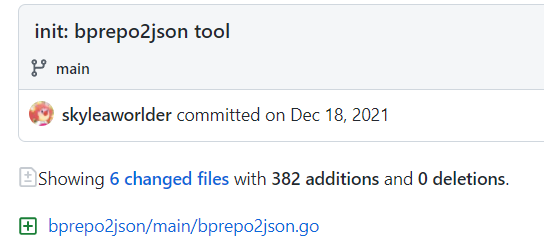
\includegraphics[width=2in]{contents/figure/pkg_repo_tool.png}
                \label{fig:pkg-repo-tool}
            \end{figure}
            \column{.5\textwidth}
            \begin{figure}
                \centering 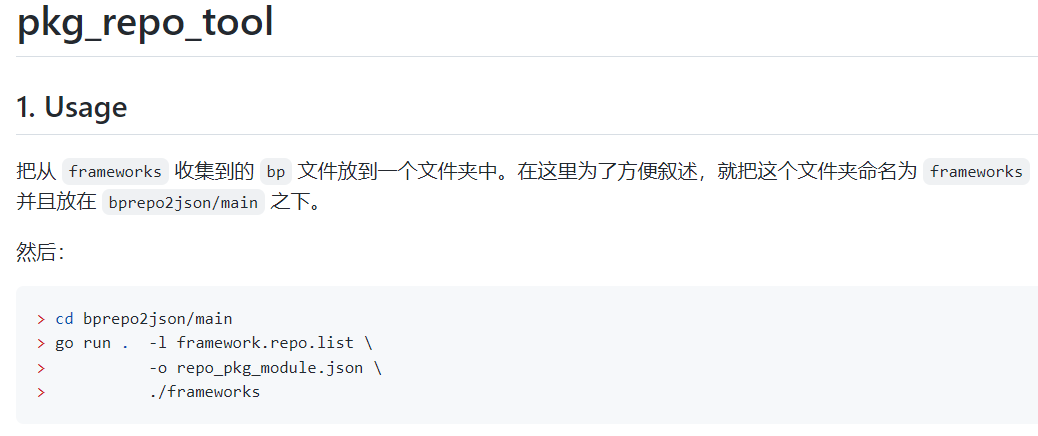
\includegraphics[width=2in]{contents/figure/pkg_repo_tool_readme.png}
                \label{fig:pkg-repo-tool-readme}
            \end{figure}
        \end{columns}
    \end{frame}

    % “简单公式” 示例
    \begin{frame}{软件变更的获取}
        \begin{block}{git diff 的读取}
            通过给定的两个提交 Hash ID,借助开源工具 jgit 使用 kotlin 抽象并结构化源文件差异。\cite{diff-extractor}得到从变更文件到存在变更的类内方法的映射关系。(待完善)
        \end{block}
        \begin{figure}
            \centering 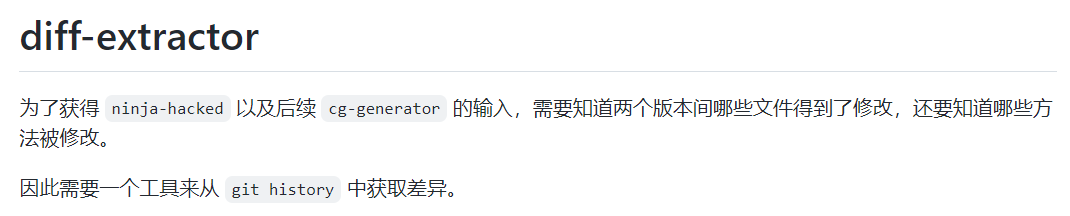
\includegraphics[width=4.3in]{contents/figure/diff_extractor_readme.png}
            \label{fig:diff-extractor-readme}
        \end{figure}
    \end{frame}

    \begin{frame}{模块间分析}
        \begin{block}{基于 AOSP 底层构建系统 ninja 的文件依赖关系分析}
            \small ninja 中使用 “rule” 与 “build” 抽象和实例化构建过程。通过对 ninja 已有数据结构的利用,使用 C++ 编写适配 ninja 的工具 “OriginTool”,得到变更节点影响的所有节点。\cite{ninja-hacked}
        \end{block}
        \begin{block}{依赖关系有向无环图生成}
            \small 借助开源工具 graphviz (in javascript) 提供的对节点的抽象,对 ninja “OriginTool” 的输出文件进行可视化。\cite{deps-reflector}
        \end{block}

        \begin{columns}
            \column{.5\textwidth}
            \begin{figure}
                \centering 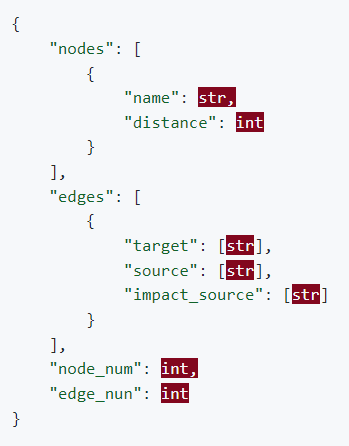
\includegraphics[width=1.2in, height=1in]{contents/figure/ninja_hacked_output.png}
                \label{fig:ninja-hacked-output}
            \end{figure}
            \column{.5\textwidth}
            \begin{figure}
                \centering 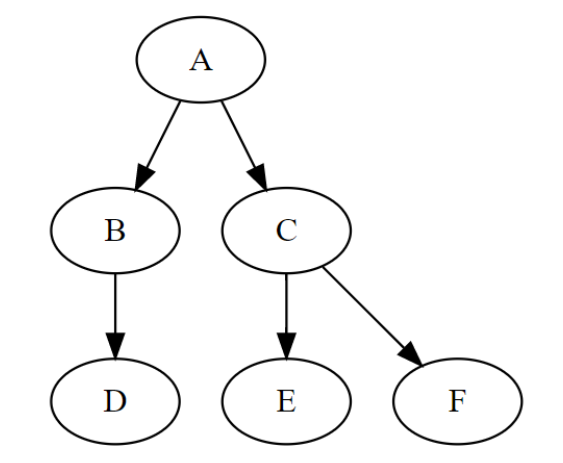
\includegraphics[width=1.8in, height=1in]{contents/figure/ninja_logic.png}
                \label{fig:ninja-logic}
            \end{figure}
        \end{columns}
    \end{frame}

    \begin{frame}{模块内分析}
        \begin{block}{调用图的生成}
            \small 使用程序间分析作为 AOSP Frameworks 模块内分析的主要途径。
            借助 JVM 字节码操作库 bcel,使用 Java 对 jar 内部 class 文件中字段的读取,找到方法声明及调用点,跨 class 文件构建方法调用图。\cite{cg-generator}
        \end{block}
        \begin{figure}
            \centering 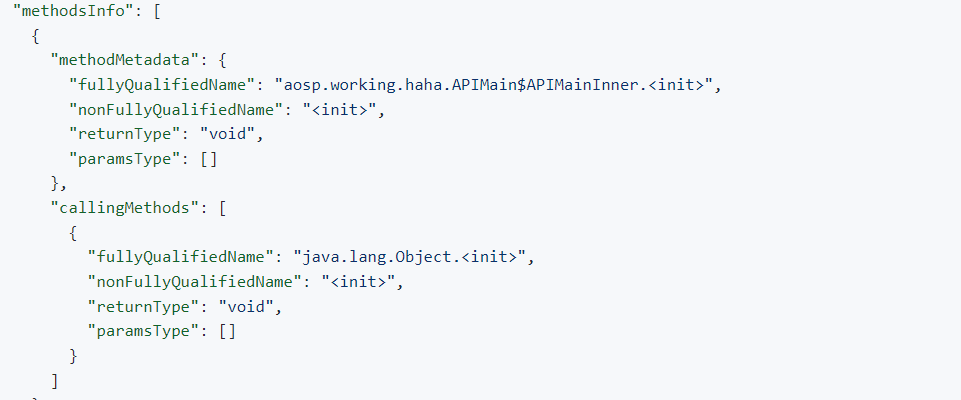
\includegraphics[width=4in]{contents/figure/cg_generator_output.png}
            \label{fig:cg-genrator-output}
        \end{figure}
    \end{frame}
